% !TEX options=--shell-escape
\documentclass[usenames,dvipsnames,9pt]{beamer}
\usetheme{metropolis}

\usepackage[czech]{babel}
\selectlanguage{czech}

\usepackage{hyperref}
\usepackage{fontawesome}
\usepackage{minted}
\usepackage{mathtools}
\usepackage{tabularx}
\usepackage{smartdiagram}
\usepackage{qrcode}

\newcommand{\download}[1]{\hfill\faDownload\hspace{5pt}\href{https://cw.fel.cvut.cz/wiki/_media/courses/be4m36mas/#1}{\tt #1}\\[1.3em]}
\newcommand{\see}[1]{\faEye\hspace{5pt}#1}
\newcommand{\sep}{\hspace{10pt}/\hspace{10pt}}


% Generate frame with QR code to a feedback form.
\newcommand{\framefeedback}[1]{
  \begin{frame}[standout]
    \begin{minipage}{0.4\linewidth}
      \begin{center}
        \textbf{\LARGE Díky za pozornost!}
      \end{center}

      \vspace{3em}

      \raggedleft\small Budeme rádi za Vaši\\zpětnou vazbu! $\rightarrow$
    \end{minipage}
    \hfill
    \begin{minipage}{0.5\linewidth}
      \vspace{4em}
      \centering\qrcode[height=\linewidth]{#1}\\
      \vspace{0.8em}
      \url{#1}
    \end{minipage}
  \end{frame}
}


\title{Úvod do B4B36PDV}
\subtitle{Organizace předmětu a seznámení se s paralelizací}
\date{}
% \author{Karel Horák}
\institute{B4B36PDV -- Paralelní a distribuované výpočty}

\metroset{block=fill}

\begin{document}
\maketitle

\begin{frame}
  \frametitle{Osnova}
  \begin{itemize}
    \item Čím se budeme zabývat?
    \item Hodnocení předmětu\\[1.5em]
    \item Úvod do paralelního hardwaru a softwaru
  \end{itemize}
\end{frame}

\section{Organizace předmětu}

\begin{frame}
  \frametitle{Důležité informace}
  \small
  \textbf{Přednášející}: \hspace{5pt} Jakub Mareček \hspace{10pt} Michal Jakob \\[1em]
  \textbf{Cvičící}: \\
  \hspace*{10pt} \textbf{Paralelní část}: Petr Macejko, David Fiedler, Tomáš Rouček, Zdeněk Rozsypálek \\
  \hspace*{10pt} \textbf{Distribuovaná část}: Petr Macejko, Jan Mrkos, David Milec \\[3.5em]
  Důležité odkazy: \\[0.7em]
  {\Large\url{https://cw.fel.cvut.cz/wiki/courses/b4b36pdv}} \\[0.7em]
  \url{https://cw.felk.cvut.cz/forum/} \\
  \url{https://cw.felk.cvut.cz/brute/}
\end{frame}

\begin{frame}[t]
  \frametitle{Čím se budeme zabývat?}
	\begin{center}
    \Large
      \only<1,3->{Paralelní}\only<2>{\alert{Paralelní}}
      \ \ \ \ \ a \ \ \ \ \ 
      \only<1-2>{Distribuované}\only<3->{\alert{Distribuované}}
      výpočty
  \end{center}

  \metroset{block=fill}
  \begin{minipage}[t]{0.49\linewidth}
    \only<2->{
    \begin{block}{Paralelní výpočty}
      \vspace{1em}
      \begin{itemize}
        \item \textbf{Jeden} výpočet provádí současně \textbf{více} vláken
        \item Vlákna typicky sdílí pamět a výpočetní prostředky\\[1em]
        \item Cíl: Zrychlit výpočet úlohy \\[1em]
        \item {\small (7 týdnů)}
      \end{itemize}
    \end{block}}
  \end{minipage}
  \hfill
  \begin{minipage}[t]{0.49\linewidth}
    \only<3->{
    \begin{block}{Distribuované výpočty}
      \vspace{1em}
      \begin{itemize}
        \item Výpočet provádí současně více oddělených výpočetních uzlů {\small (často i geograficky)} \\[1em]
        \item Cíle:
              \begin{itemize}
                \item Zrychlit výpočet
                \item \only<3>{Robustnost výpočtu}
                      \only<4->{\alert{Robustnost výpočtu}}
              \end{itemize}\vspace{1em}
        \item {\small (6 týdnů)}
      \end{itemize}
    \end{block}}
  \end{minipage}
\end{frame}

\begin{frame}
  \frametitle{Hodnocení předmětu}
  \metroset{block=fill}
  \vspace{0.5em}
  \begin{block}{Paralelní výpočty}
    \begin{itemize}
      \item 5 malých programovacích úloh \hfill 10 bodů
      \item Semestrální práce            \hfill 12 bodů
    \end{itemize}
  \end{block}
  \begin{block}{Distribuované výpočty}
    \begin{itemize}
      \item 2 malé úlohy                 \hfill  4 body
      \item Semestrální práce            \hfill 14 bodů
    \end{itemize}
  \end{block}
  \begin{block}{Praktická zkouška}
    \begin{itemize}
      \item Praktická část zkoušky (min. 10b)          \hfill 20 bodů \\
            {\small\ \ (Vyřešení zadaného problému za použití paralelizace.)}
      \item Teoretická část zkoušky (min. 20b)         \hfill 40 bodů
    \end{itemize}
  \end{block}
  V semestru musíte získat \textbf{alespoň 20 bodů} \hfill Celkem: 100 bodů
\end{frame}
\begin{frame}
  \frametitle{Hodnocení předmětu}
  \begin{center}
    \LARGE Vyžadujeme \textbf{samostatnou} práci na všech úlohách.
  \end{center}

  \vspace{2em}

  \faWarning \hspace{3pt}
  \textbf{Plagiáty jsou zakázané.} Nepřidělávejte prosím starosti nám, ani sobě.
\end{frame}

% \begin{frame}
%   \frametitle{Pozdní odevzdání úloh}
%   Domácí úlohy budou mít \textbf{striktní} deadline, ale...

%   \begin{center}
%     \LARGE V rámci semestru máte k dispozici 7 tzv. \emph{late-days}.
%   \end{center}

%   \small
%   \begin{itemize}
%     \item Za každý den, o který se při odevzdávání úlohy opozdíte, Vám odečteme 1 den.
%     \item Pokud se v součtu opozdíte o méně jak 7 dnů, žádné body Vám nestrhneme.
%     \item V opačném případě budou některé Vaše odevzdané úlohy hodnoceny za \textbf{0 bodů}.
%           \pause
%           \begin{itemize}
%             \item Body dostanete za takovou podmnožinu odevzdaných úkolů, u kterých jste se opozdili v součtu o méně jak 7 dnů.
%             \item Tuto podmnožinu vybereme tak, abyste za úkoly v součtu dostali nejvíce bodů (tj., ve Váš prospěch).
%           \end{itemize}
%   \end{itemize}
% \end{frame}

\begin{frame}
  \frametitle{Hodnocení předmětu}
  {\Large Docházka na cvičení není povinná.}

  \hfill To ale neznamená, že byste na cvičení neměli chodit...

  \vspace{2em}

  \begin{itemize}
    \item Budeme probírat látku, která se Vám bude hodit u úkolů a u zkoušky.
    \item Dostanete prostor pro práci na semestrálních pracích.
    \item Konzultace budou probíhat \textbf{primárně} na cvičeních.
    \item Ušetříme Vám čas a nervy (nebo v to alespoň doufáme ;-)
  \end{itemize}

  \vfill\hrule
  \small
  \faWarning \hspace{3pt}
  Pokud se na cvičení rozhodnete nechodit, budeme předpokládat, že probírané látce dokonale rozumíte.
  Případné konzultace v žádném případě nenahrazují cvičení!
\end{frame}

\begin{frame}
  \frametitle{Na čem budeme stavět?}
  \begin{itemize}
    \item Programování v jazyce C/C++ {\small (B0B36PRP)}
          \begin{itemize}
            \item Základy programování v jazyce C/C++
            \item Kompilace programů v jazyce C/C++
            \item Základy objektového programování (znalost C++11 výhodou)
          \end{itemize}
    \pause
    \item Technologické předpoklady paralelizace {\small (B4B36OSY)}
          \begin{itemize}
            \item Vlákna a jejich princip
            \item Metody synchronizace a komunikace vláken
          \end{itemize}
    \pause
    \item Základní znalost fungování počítače a procesoru {\small (B4B35APO)}
    \pause
    \item Znalost základních algoritmů {\small (B4B33ALG)}
  \end{itemize}
\end{frame}

\section{Opakování}
\begin{frame}
  \frametitle{Kompilace programů v C/C++ s pomocí Cmake}
  \download{tutorial\_01.zip}
  \begin{block}{Vygenerování build scriptů}
    \texttt{cmake <src dir>}
  \end{block}
  Zde \texttt{<src dir>} je složka se souborem \texttt{CMakeLists.txt}.
  \vspace{1em}
  \begin{block}{Kompilace}
    \texttt{cmake --build <build dir>}
  \end{block}
  Zde \texttt{<build dir>} je složka s vygenerovanými soubory pro sestavení programu.

  Nebo použijte IDE s dobrou podporou C++, například CLion (multiplatformní) nebo Visual Studio (Windows)
\end{frame}

\begin{frame}
  \frametitle{Bylo, nebylo...}
  Pro připomenutí: Cílem paralelních výpočtů je dosáhnout zvýšení výkonu
  \vfill
  \begin{minipage}{0.3\linewidth}
    \centering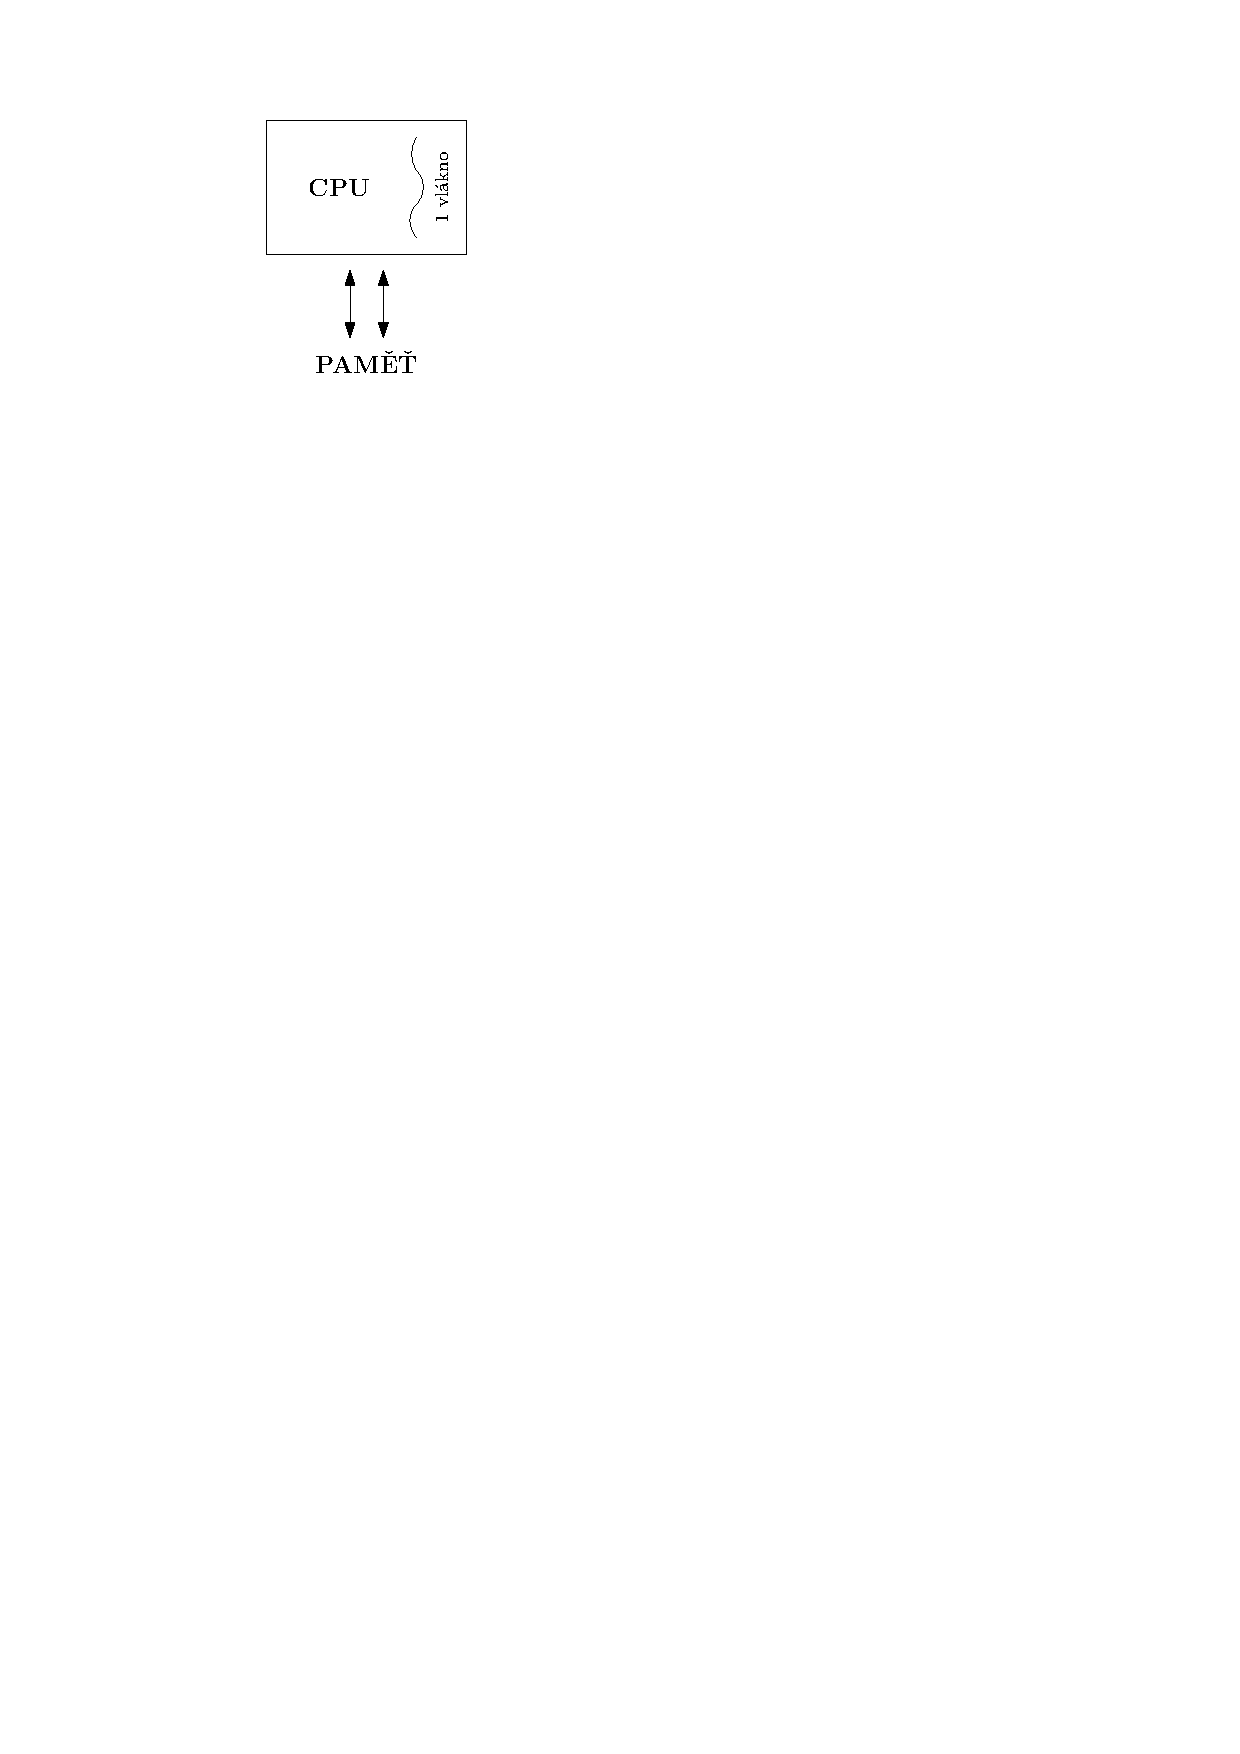
\includegraphics[width=0.7\linewidth]{01/figs/single_thread.pdf}
  \end{minipage}
  \hfill
  \begin{minipage}{0.6\linewidth}
    \textbf{\underline{von Neumannova architektura}}
    \begin{itemize}
      \item Jaké má nevýhody?
      \item Jak bychom je mohli opravit?
      \item A jak bychom dále mohli navýšit výkon procesoru?
    \end{itemize}
    \vspace{1em}
    \see{{\tt memory.cpp}}
  \end{minipage}

  \vspace{3em}

  \pause
  \alert{
    \Large
    Vyzkoušejte si prosím, že Vám funguje přístup do BRUTE a odevzdejte soubor \texttt{memory.cpp}.
  }
\end{frame}
\begin{frame}
  \frametitle{Moderní procesor}
  \centering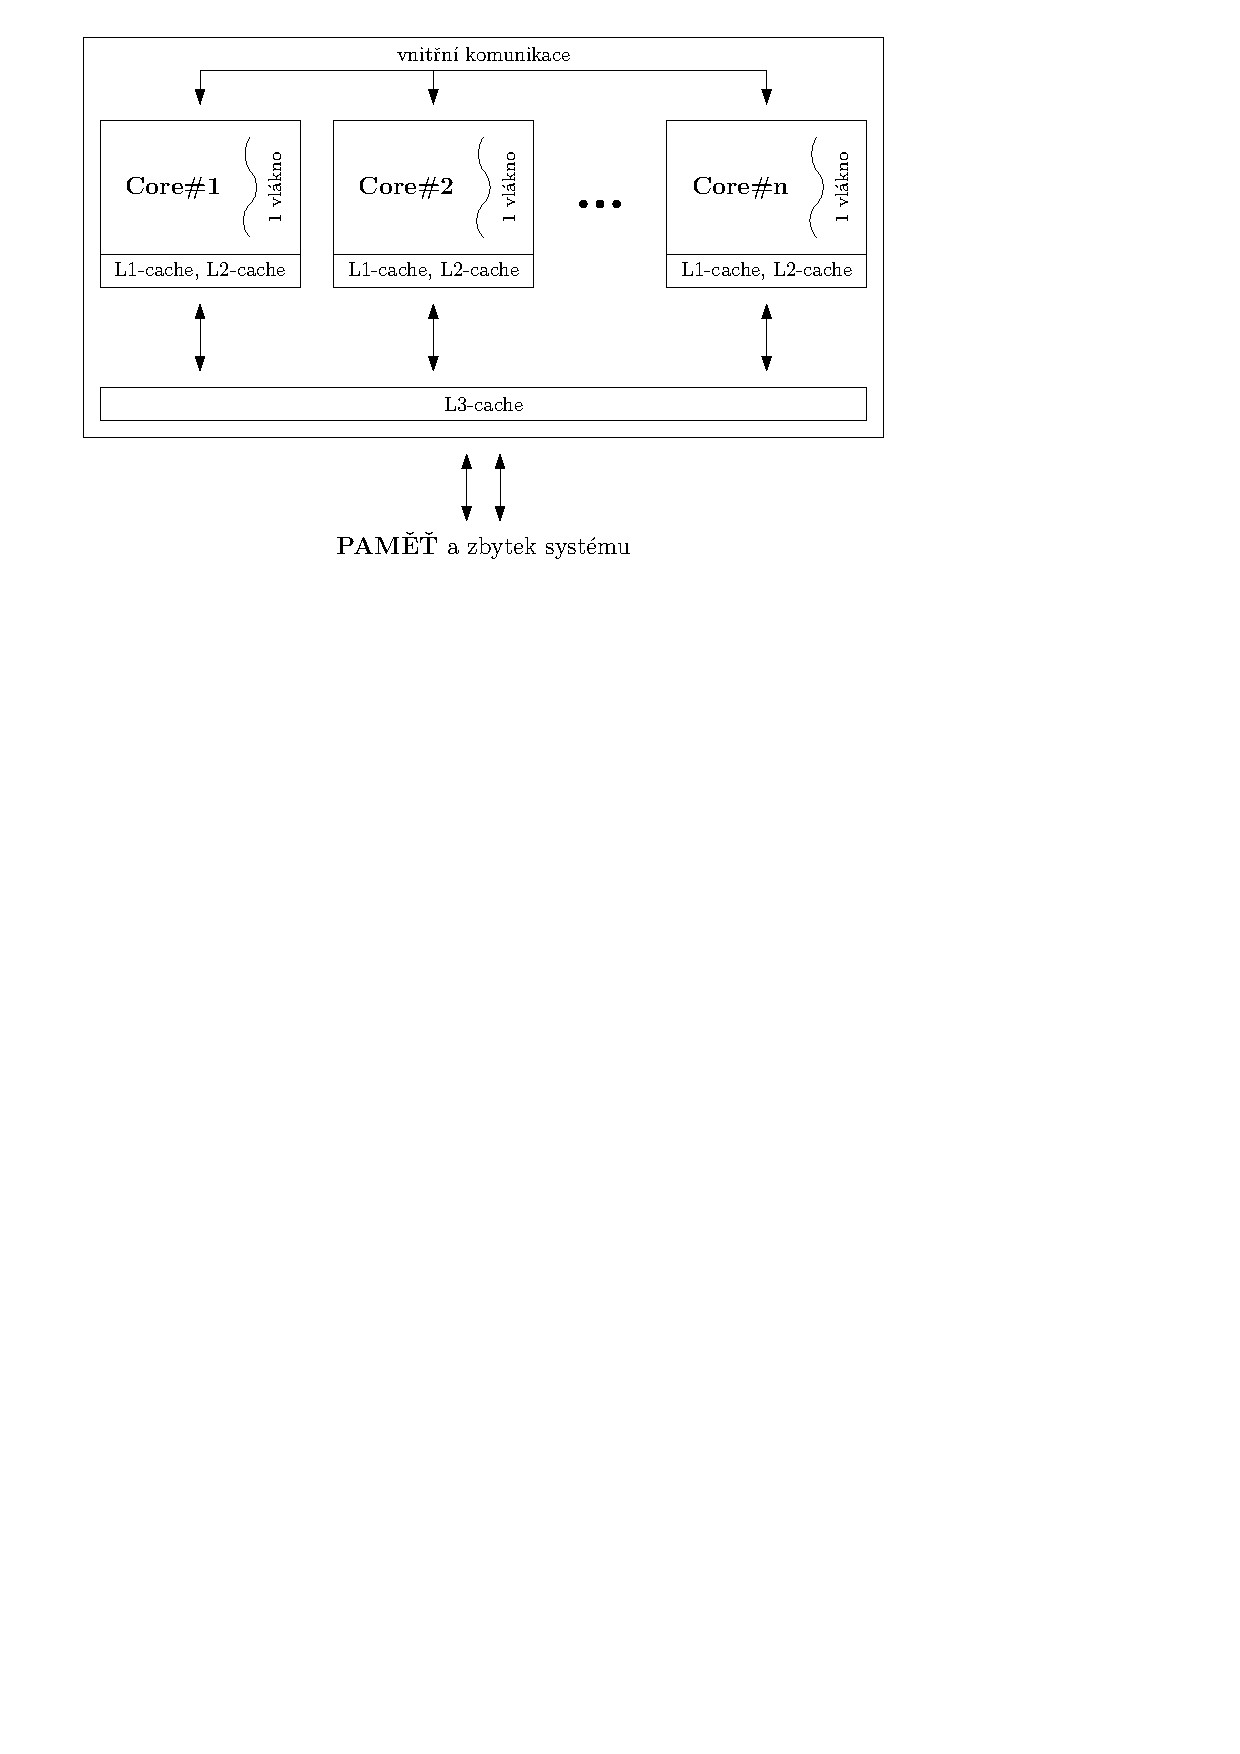
\includegraphics[width=0.8\linewidth]{01/figs/modern_cpu.pdf}
\end{frame}
\begin{frame}[t]
  \frametitle{Moderní procesor}
  \centering
  \smartdiagramanimated[bubble diagram]{Paralelizace,
    Pipelining \\ {\footnotesize (procesor)},
    Vektorizace \\ {\footnotesize (kompilátor)},
    Vlákna \\ {\footnotesize (Vy :-)}}
\end{frame}
\begin{frame}
  \frametitle{Moderní procesor}
  Možné ``nástrahy'' použití moderního procesoru s více jádry a cache:
  \begin{itemize}
    \item Komunikace s pamětí je stále pomalá (problém \emph{cache-miss})
    \item Přístup ke sdíleným datům více vlákny (\emph{true sharing})
    \item Udržování koherence cache může být drahé (\emph{false sharing}) \\[2em]
    \item ... a jiné
  \end{itemize}
\end{frame}

\begin{frame}
  \frametitle{Cache-miss}

  \see{\tt{memory.cpp}}

  \vspace{2em}

  \see{\tt{matrix.cpp}}
\end{frame}

\begin{frame}[fragile]
  \frametitle{True sharing}
  \begin{minted}{c}
    void multiply(int* number, int multiplyBy) {
      *number = (*number) * multiplyBy;
    }
  \end{minted}
  \vspace{1.5em}
  Předpokládejme \mintinline{c}{int number = 1;} a mějme dvě vlákna:
  \begin{itemize}
    \item Vlákno 1: \mintinline{c}{multiply(&number,2)}
    \item Vlákno 2: \mintinline{c}{multiply(&number,3)}
  \end{itemize}
  Co bude v proměnné \mintinline{c}{number} po skončení obou vláken?
\end{frame}
\begin{frame}[fragile]
  \frametitle{True sharing}
  \begin{minted}{c}
    void multiply(int * number, int multiplyBy) {
      *number = (*number) * multiplyBy;
    }
  \end{minted}
  \vspace{1em}\[ \Bigg\downarrow \]\vspace{1em}
  \begin{minted}{gas}
    imul esi, DWORD PTR [rdi]
    mov DWORD PTR [rdi], esi
    ret
  \end{minted}

  \pause

  \vspace{1.5em}
  {\hfill\see{\url{http://godbolt.org}}}
\end{frame}
\begin{frame}[t,fragile]
  \frametitle{True sharing}
  \begin{minipage}[t]{0.45\linewidth}
    Vlákno 1 \sep\mintinline{gas}{mov esi, 2}\\[-0.5em]
    \hrule\vspace{0.5em}

    \footnotesize
    \only<4-5>{\vspace{4em}}%
    \mintinline{gas}{imul esi, DWORD PTR [rdi]}\only<6-7>{\vspace{2em}}\only<8->{\vspace{4.5em}}\\
    \mintinline{gas}{mov DWORD PTR [rdi], esi}\\
    \mintinline{gas}{ret}
    \only<4-5>{\vspace{0.5em}}
  \end{minipage}
  \hfill
  \begin{minipage}[t]{0.45\linewidth}
    Vlákno 2 \sep\mintinline{gas}{mov esi, 3}\\[-0.5em]
    \hrule\vspace{0.5em}

    \footnotesize
    \only<2-3>{\vspace{4em}}%
    \only<6->{\vspace{1.5em}}%
    \mintinline{gas}{imul esi, DWORD PTR [rdi]}\only<6-7>{\vspace{3em}}\\
    \mintinline{gas}{mov DWORD PTR [rdi], esi}\\
    \mintinline{gas}{ret}
    \only<2-3>{\vspace{0.5em}}
  \end{minipage}

  \begin{center}
    \vfill\only<3,5,7,9>{Výsledek:\hspace{20pt}}%
    \tt
    \only<3,5>{number = 6}%
    \only<7>{number = 3}%
    \only<9>{number = 2}%
  \end{center}
  \only<10>{
    \vspace{1em}\hrule
    \small Jaké máme možnosti, abychom dosáhli deterministického výsledku (který pravděpodobně chceme)?
  }
\end{frame}

\begin{frame}[t]
  \frametitle{False-sharing}
  Moderní procesor pracuje s pamětí \emph{po blocích}, které se mapují do cache.
  \begin{itemize}
    \item I když vlákna nepracují se stejnými proměnnými, mohou chtít pracovat se stejným \emph{blokem}.
    \item Jeden blok se pak nutně musí nacházet v cachích různých jader -- a ve více kopiích
  \end{itemize}
  \vspace{1em}
  \begin{figure}
    \centering
    \only<1>{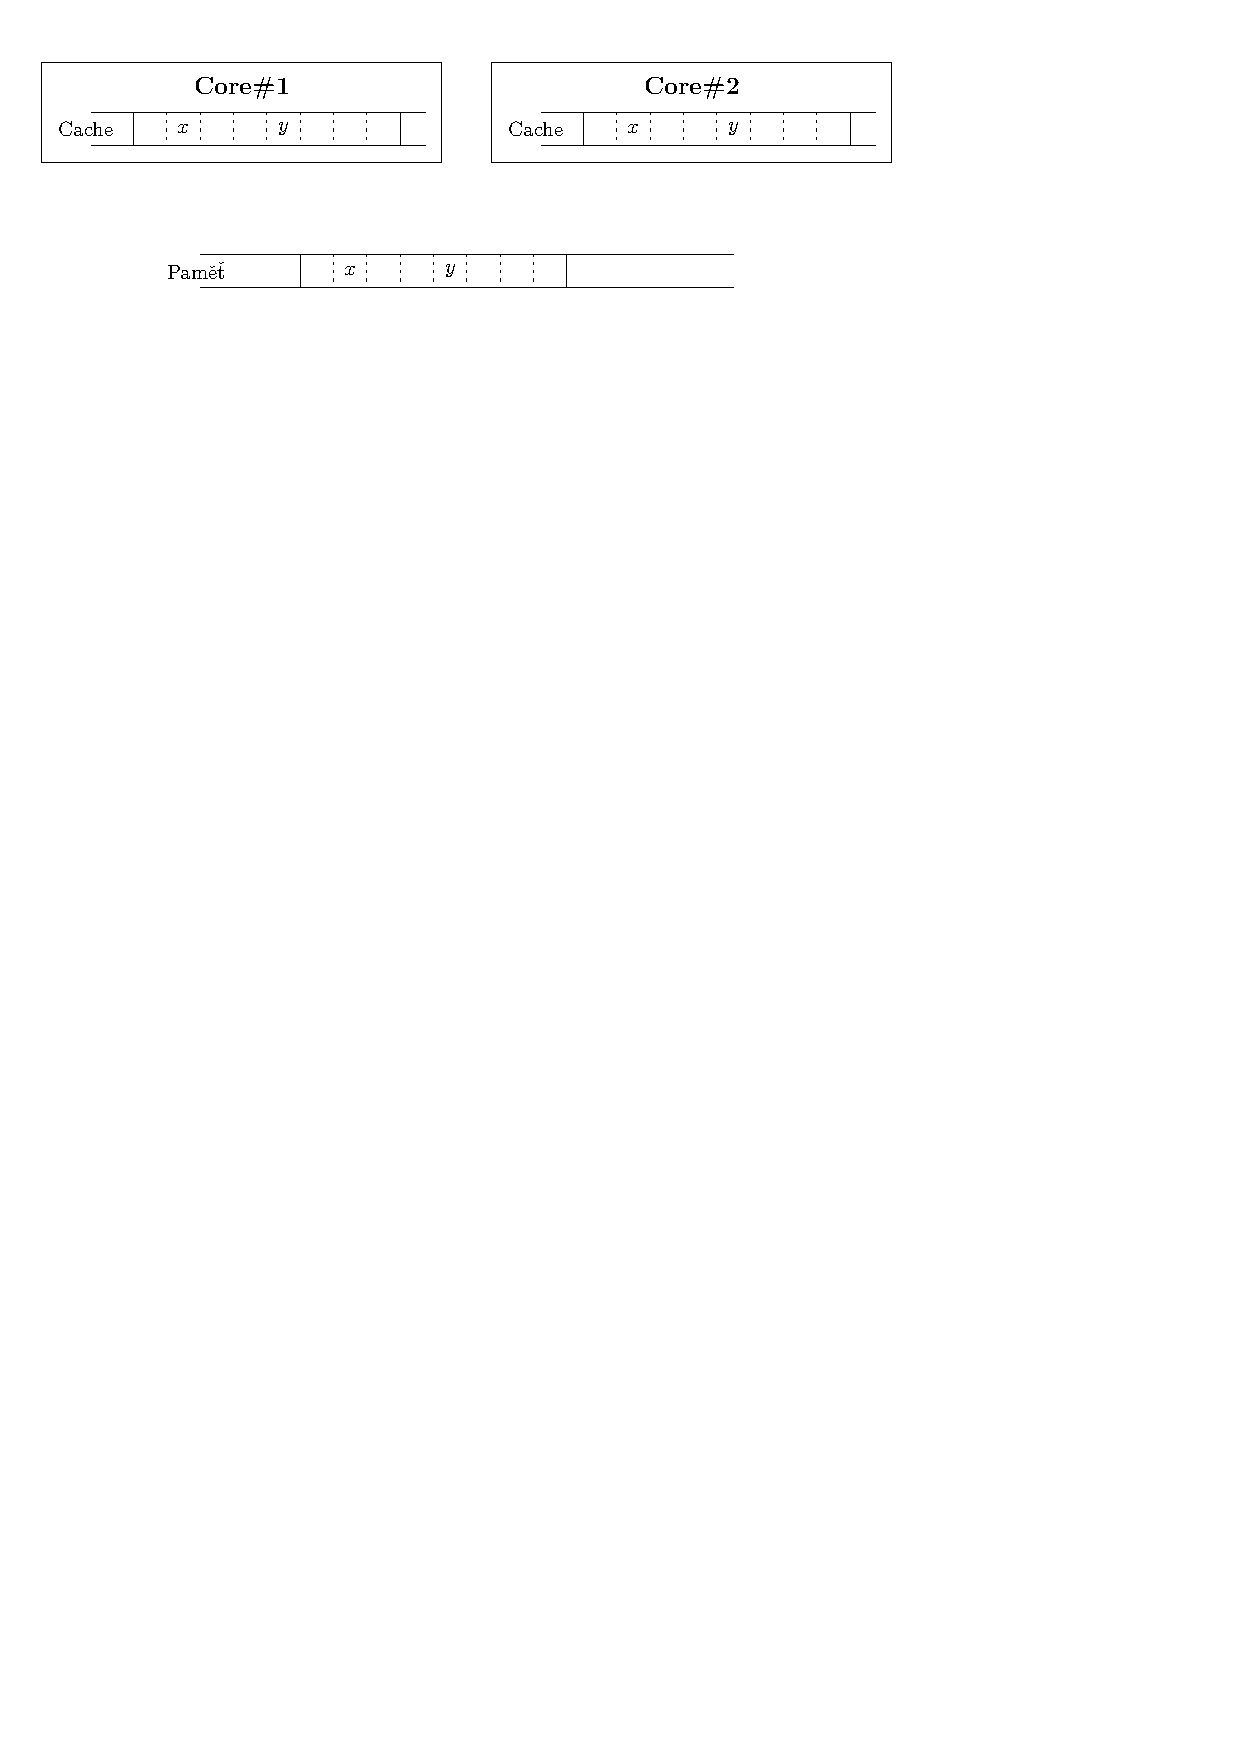
\includegraphics[width=0.8\linewidth]{01/figs/false_sharing_1.pdf}}%
    \only<2>{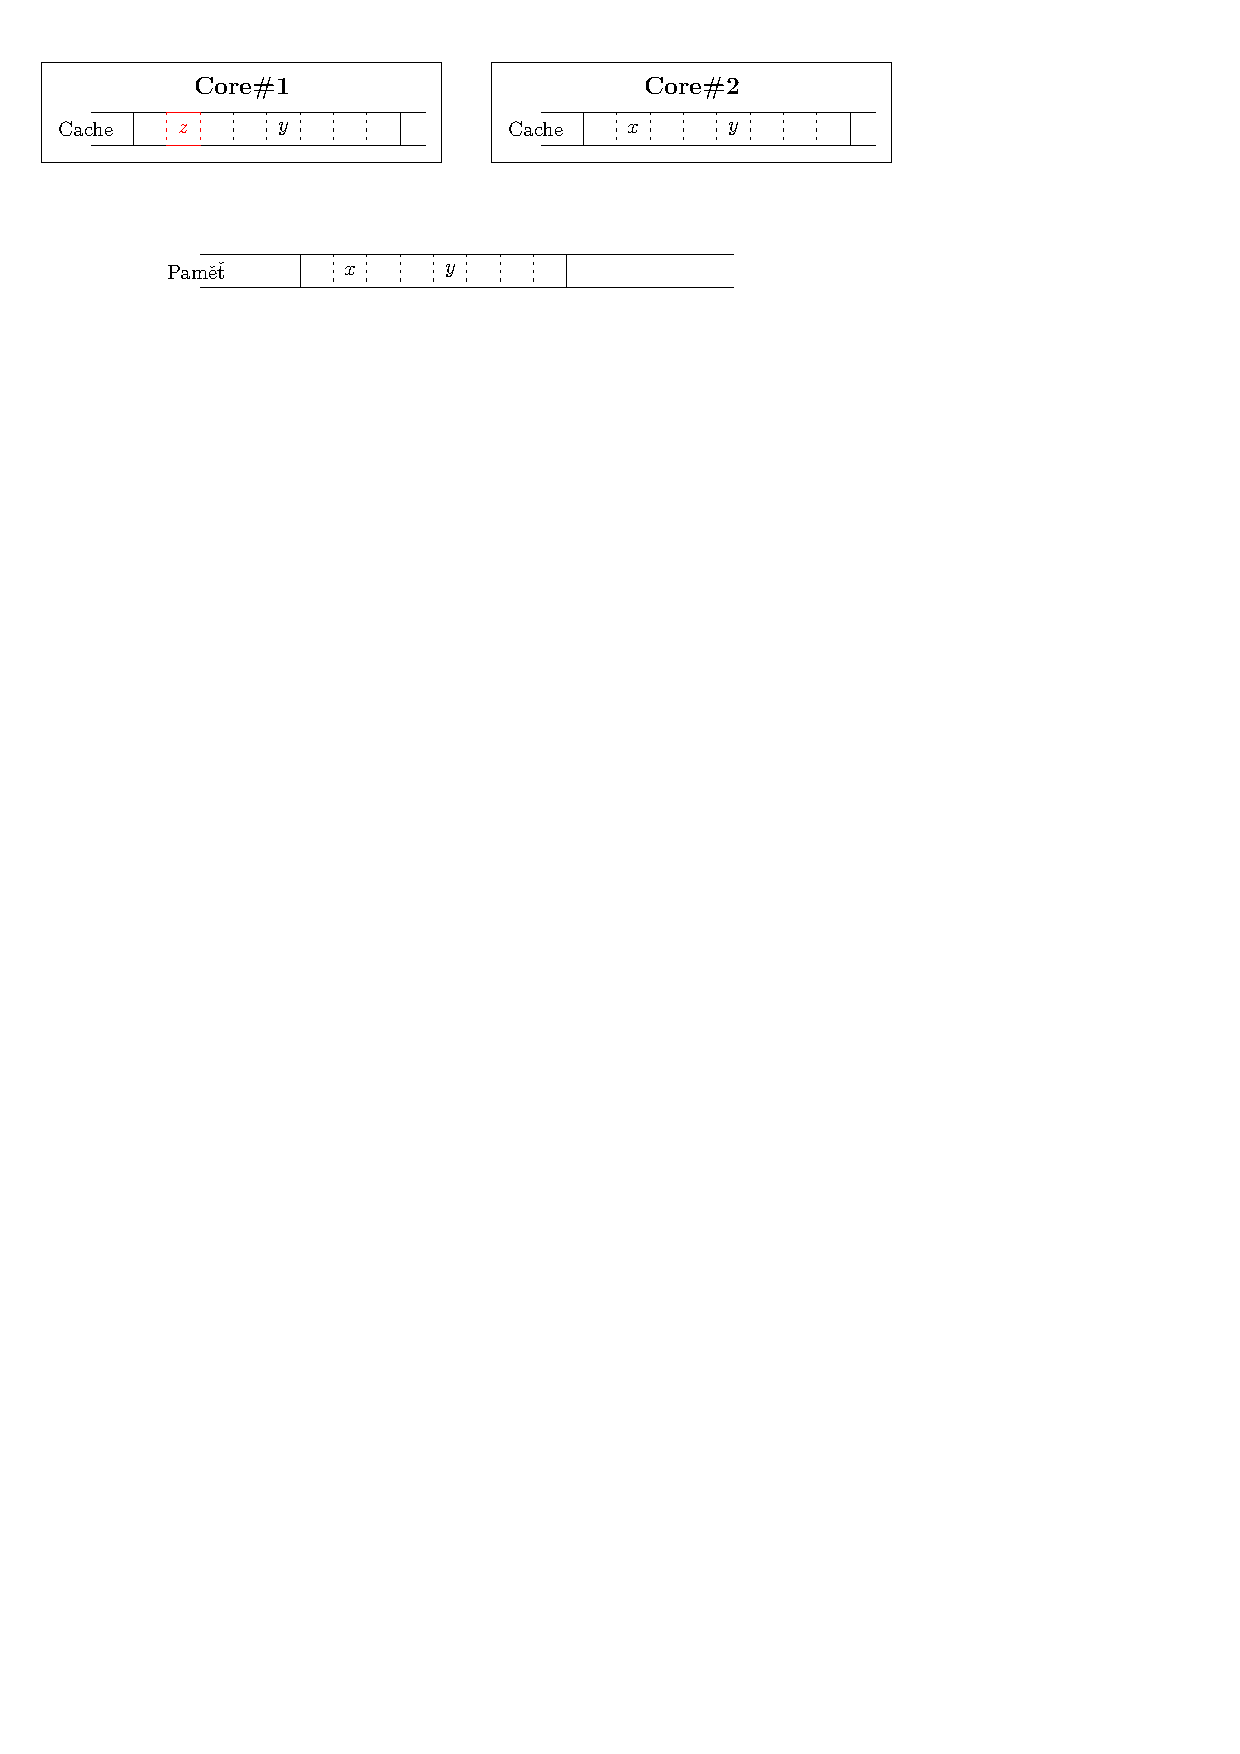
\includegraphics[width=0.8\linewidth]{01/figs/false_sharing_2.pdf}}%
    \only<3>{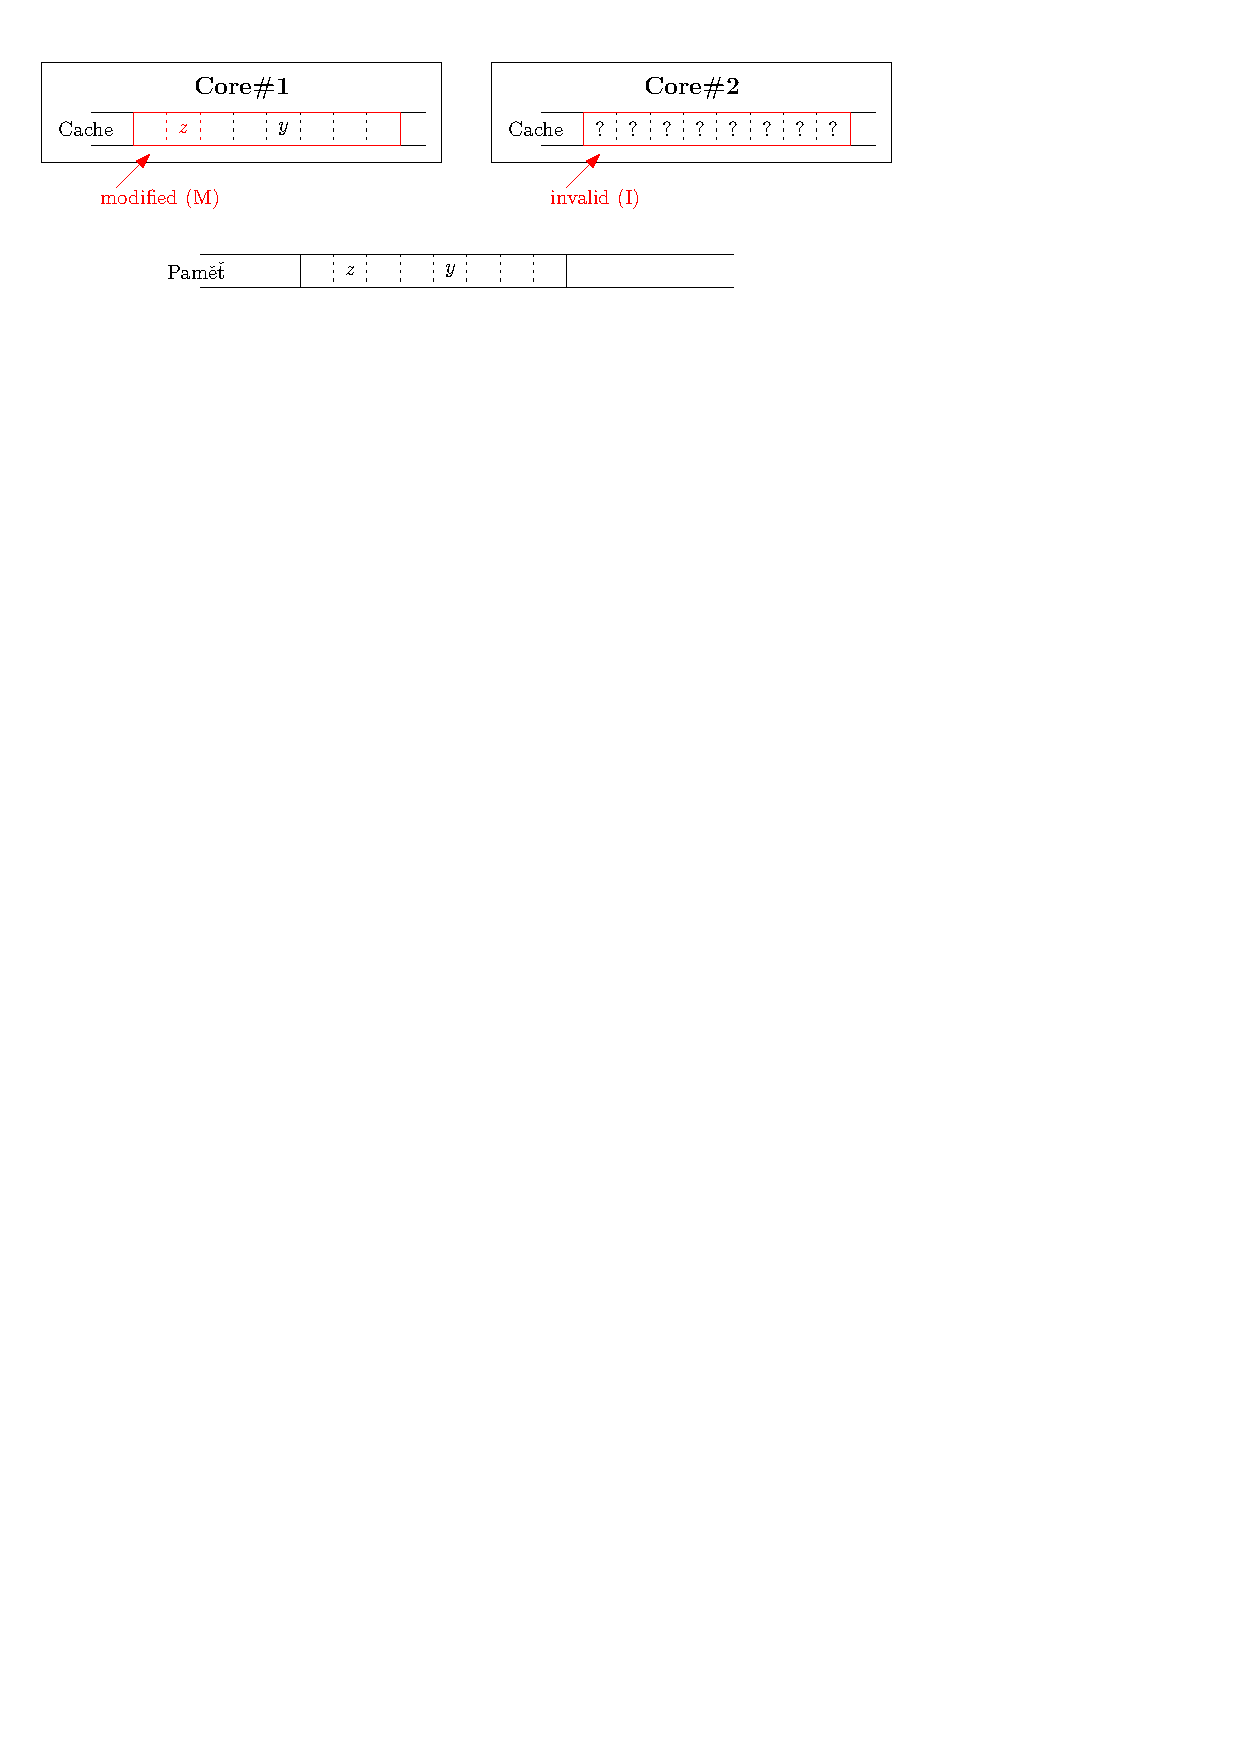
\includegraphics[width=0.8\linewidth]{01/figs/false_sharing_3.pdf}}%
    \only<4>{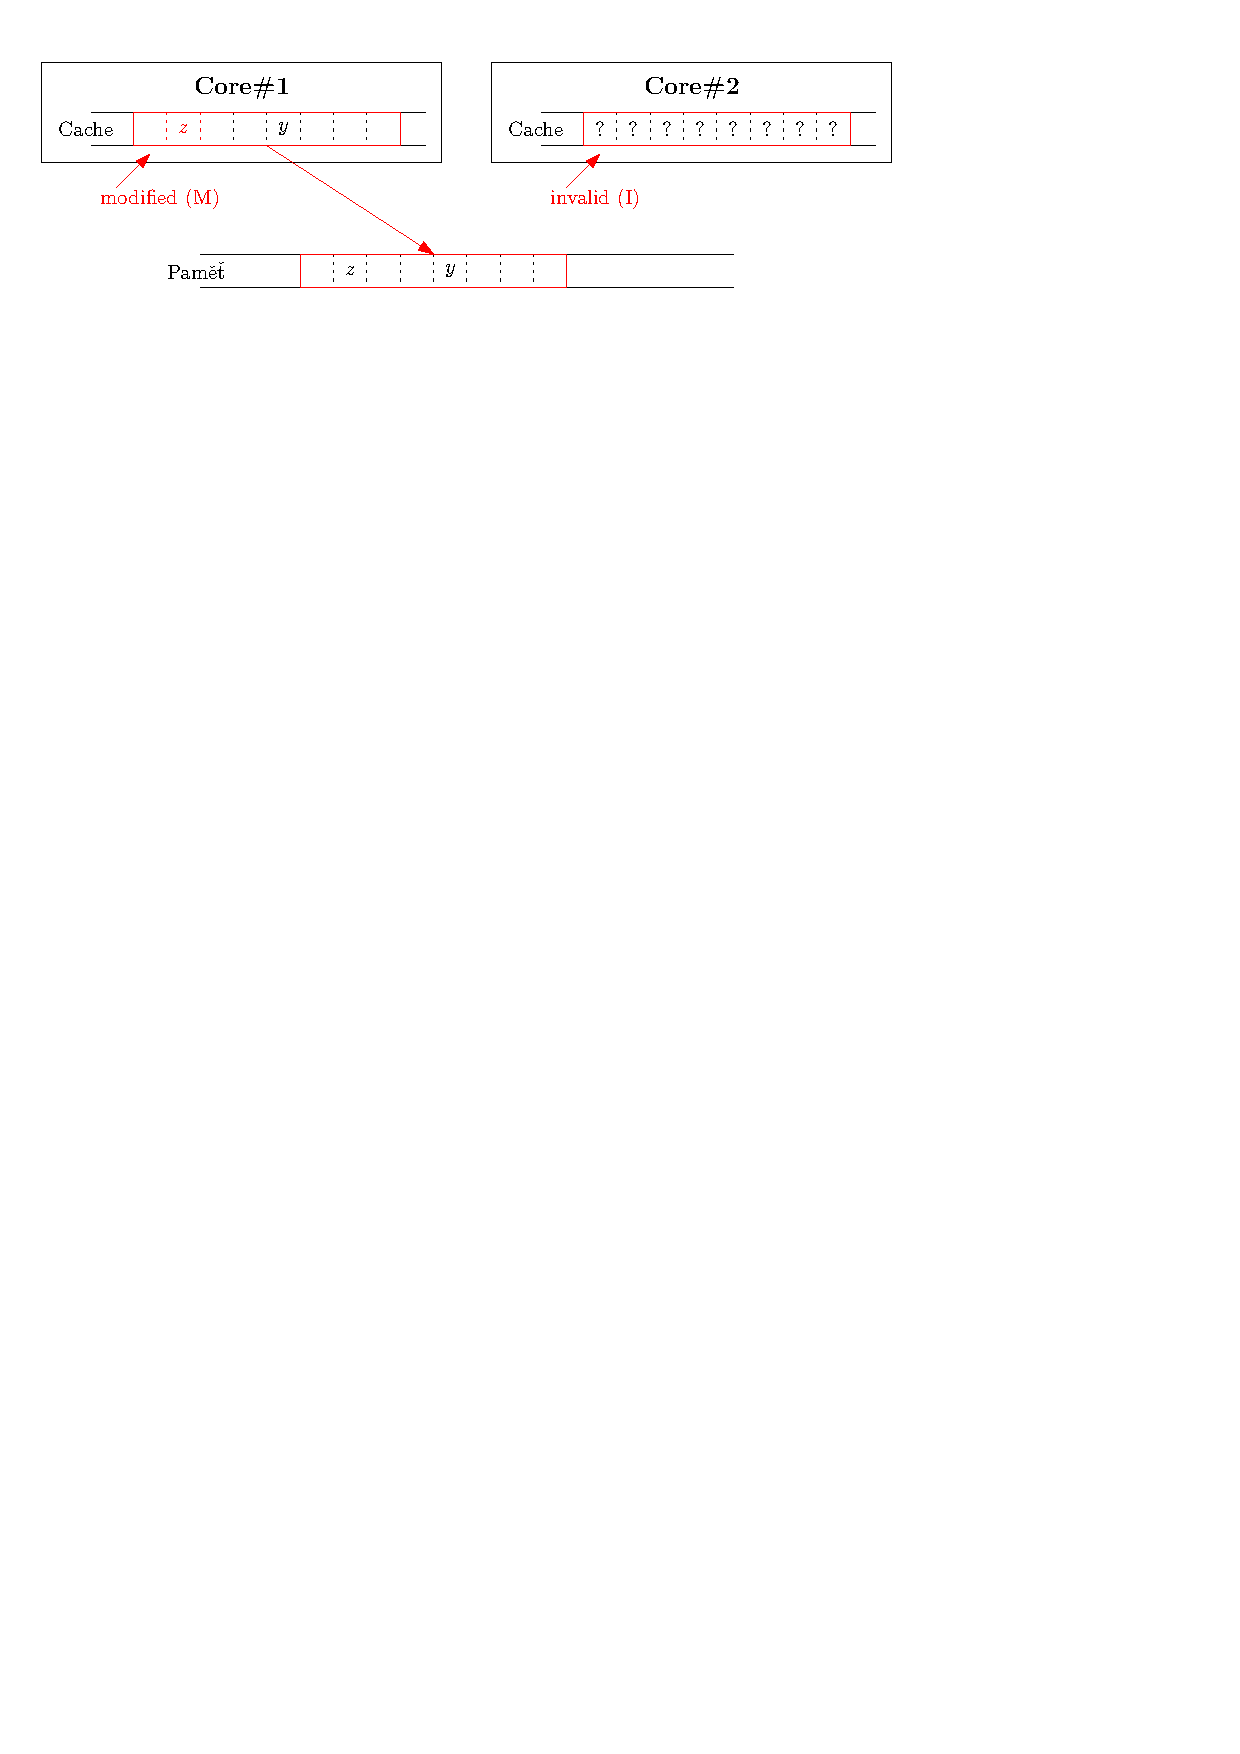
\includegraphics[width=0.8\linewidth]{01/figs/false_sharing_4.pdf}}%
    \only<5->{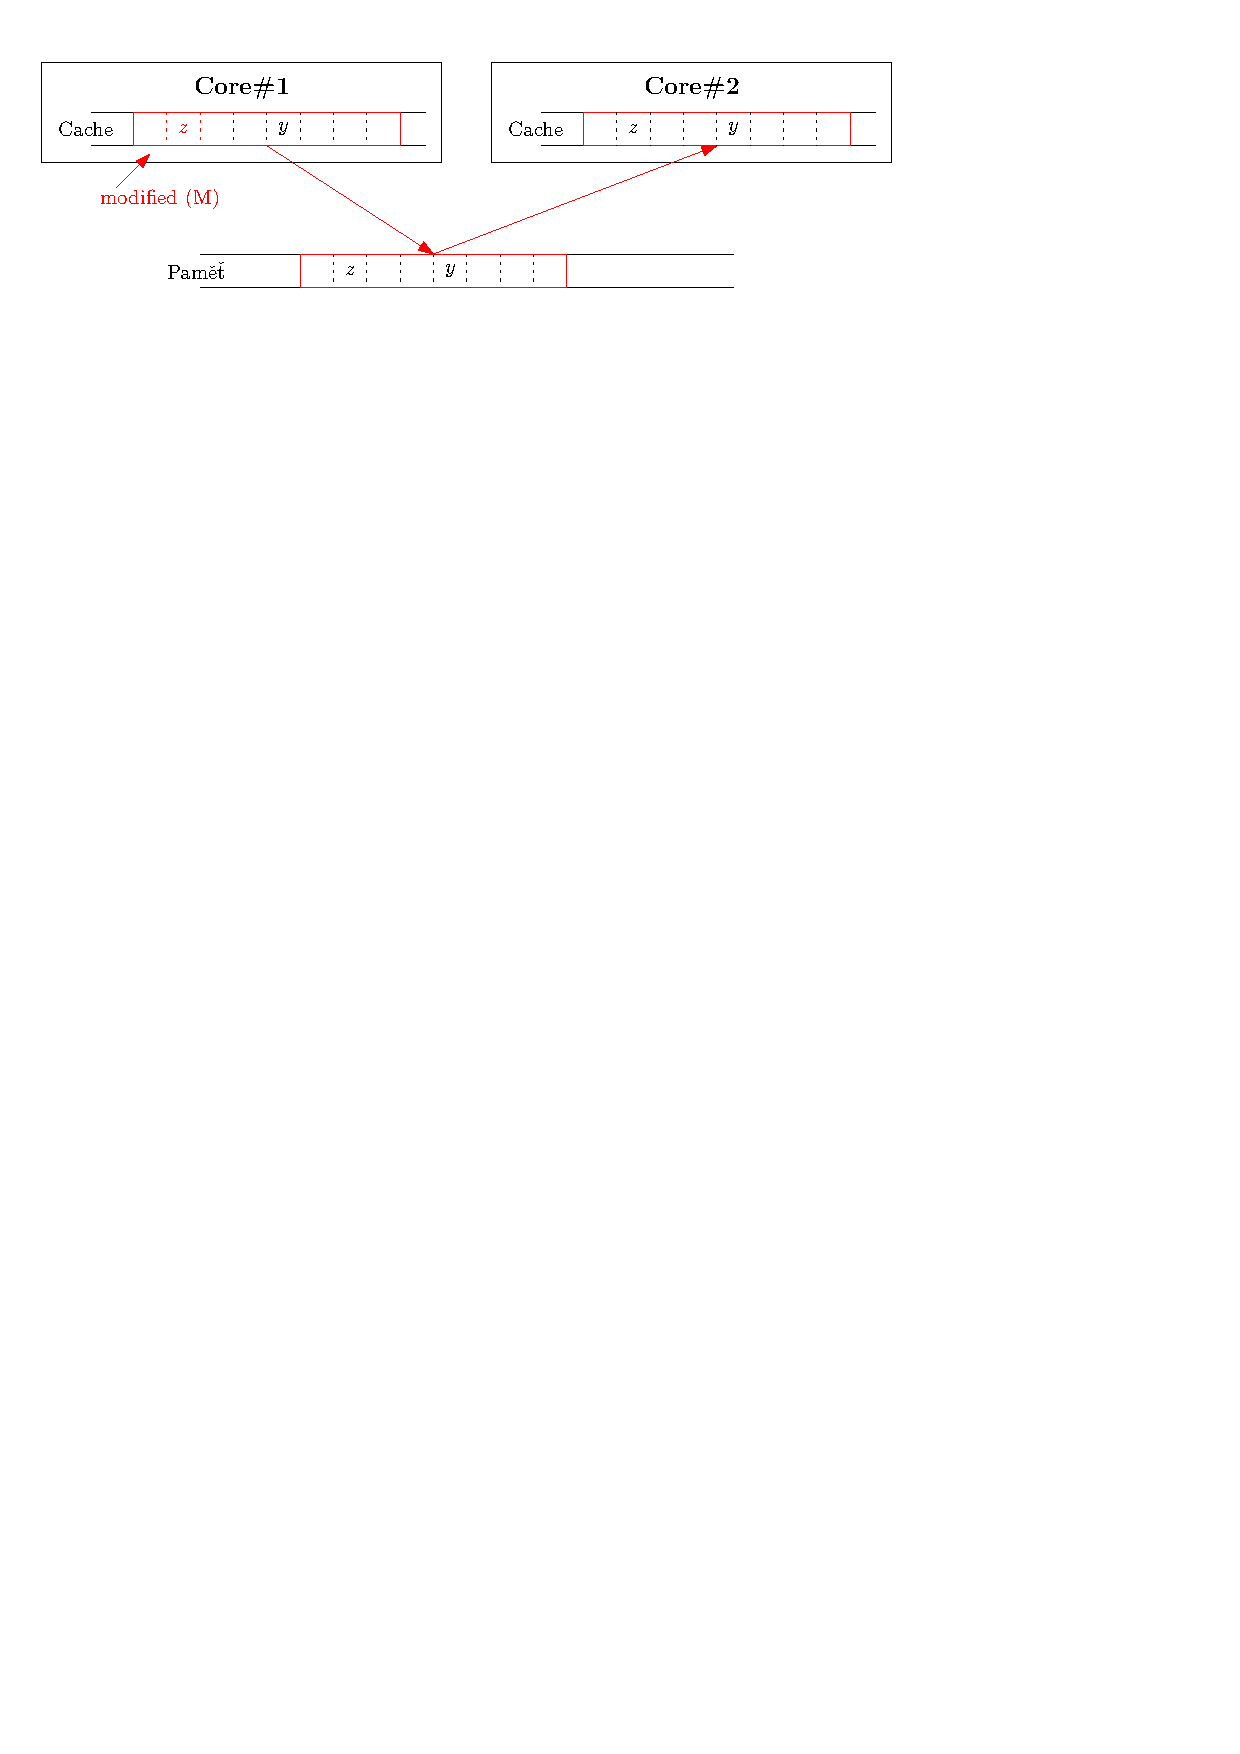
\includegraphics[width=0.8\linewidth]{01/figs/false_sharing_5.pdf}}%
  \end{figure}
  \vspace{1em}
  \begin{itemize}
    \item<6-> Ale právě té komunikaci s pamětí jsme se chtěli použitím cache vyhnout!
  \end{itemize}
\end{frame}
\begin{frame}{False-sharing}
  \centering\see{{\tt false\_sharing.cpp}}
\end{frame}

\section{Paralelizace v praxi}
\begin{frame}
  \begin{block}{Je následující tvrzení pravdivé?}
    Mějme procesor s $p$ jádry a úlohu, která při využití jednoho jádra trvá $T$ milisekund.
    Využijeme-li všech $p$ jader pro vyřešení úlohy, vyřešení úlohy zvládneme za $T/p$ milisekund.
  \end{block}
  \pause
  \textcolor{BrickRed}{\bf Tvrzení není pravdivé.} Proč? Zkuste vymyslet co možná nejvíce důvodů, proč tomu tak není.

  \pause\vspace{1.5em}
  O úlohách, kde toto tvrzení platí říkáme, že jsou tzv. \emph{lineární} nebo také \emph{embarassingly parallel}. Takových úloh ale v praxi potkáme velmi málo.
\end{frame}

{
\setbeamertemplate{frame footer}{\see{{\tt magic.cpp}}}
\begin{frame}[fragile,t]
  \vspace{1em}
  \begin{block}{Je následující tvrzení pravdivé?}
    Mějme pole o 1,000,000 prvků.
    S každým prvkem pole máme za úkol 100$\times$ provést ``magickou operaci'' $x \gets e^{\ln x}$.
    Tuto úlohu lze dobře paralelizovat.

    \begin{minted}[fontsize=\footnotesize]{c}
      void magic_operation(double * array) {
        for(unsigned int i = 0 ; i < 1000000 ; i++) {
          for(unsigned int k = 0 ; k < 500 ; k++) {
            array[i] = exp(log(array[i]));
          }
        }
      }
    \end{minted}
  \end{block}
  \pause
  \textcolor{OliveGreen}{\bf Tvrzení je pravdivé.}
  Jednotlivé výpočty hodnot \mintinline{c}{array[i]} na sobě nezávisí a můžeme je rozložit mezi různá vlákna a dosáhnout téměř lineárního nárůstu výkonu.

  \pause
  \vspace{1em}
  \hrule

  \footnotesize
  A nebo bychom si mohli vzpomenout, že $\ln x$ a $e^x$ jsou inverzní funkce.
  Ale to bychom neměli co paralelizovat ;-)
\end{frame}
\begin{frame}[fragile,t]
  \vspace{1em}
  \begin{block}{Je následující tvrzení pravdivé?}
    Mějme pole o 1,000,000 prvků.
    S každým prvkem pole máme za úkol 100$\times$ provést ``magickou operaci'' $x \gets e^{\ln x}$.
    Tuto úlohu lze dobře paralelizovat.

    \begin{minted}[fontsize=\footnotesize]{c}
      void magic_operation(double * array) {
        for(unsigned int i = 0 ; i < 1000000 ; i++) {
          for(unsigned int k = 0 ; k < 500 ; k++) {
            array[i] = exp(log(array[i]));
          }
        }
      }
    \end{minted}
  \end{block}
  
  Proč jsme ale nedosáhli $s$-násobného zrychlení (kde $s$ je počet jader procesoru?).
  Vzpomeňte si na Amdahlův zákon.
  \[ S = \cfrac{1}{(1-p) + \frac{p}{s}} \]
  Dokážete říct, co tvoří neparalelizovatelnou část programu? (vyžadující $(1-p)\%$ času)
\end{frame}
}

\iffalse
{
\setbeamertemplate{frame footer}{\see{{\tt trivial.cpp} \sep {\tt make trivial}}}
\begin{frame}[fragile]
  \begin{block}{Je následující tvrzení pravdivé?}
    Mějme pole o 1,000,000 prvků.
    S každým prvkem pole máme za úkol 100$\times$ provést ``triviální operaci'' $x \gets x + 1$.
    Tuto úlohu lze dobře paralelizovat.

    \begin{minted}[fontsize=\footnotesize]{c}
      void trivial_operation(double * array) {
        for(unsigned int i = 0 ; i < 1000000 ; i++) {
          array[i]++;
        }
      }
    \end{minted}
  \end{block}
  \pause
  \textcolor{BrickRed}{\bf Tvrzení není pravdivé.}
  Vzpomeňte si na Amdahlův zákon.
  \[ S = \cfrac{1}{(1-p) + \frac{p}{s}} \]
  Dokážete říct, co tvoří neparalelizovatelnou část programu? (vyžadující $(1-p)\%$ času)
\end{frame}
}
\fi

{\setbeamertemplate{frame footer}{\see{{\tt PDVCrypt.cpp},\ \ \ {\tt decrypt.cpp}} \hfill \faDownload \hspace{5pt} \texttt{decrypt\_data.zip}}
\begin{frame}[fragile]
  \frametitle{Šifra \texttt{PDVCrypt}}
  \begin{center}
    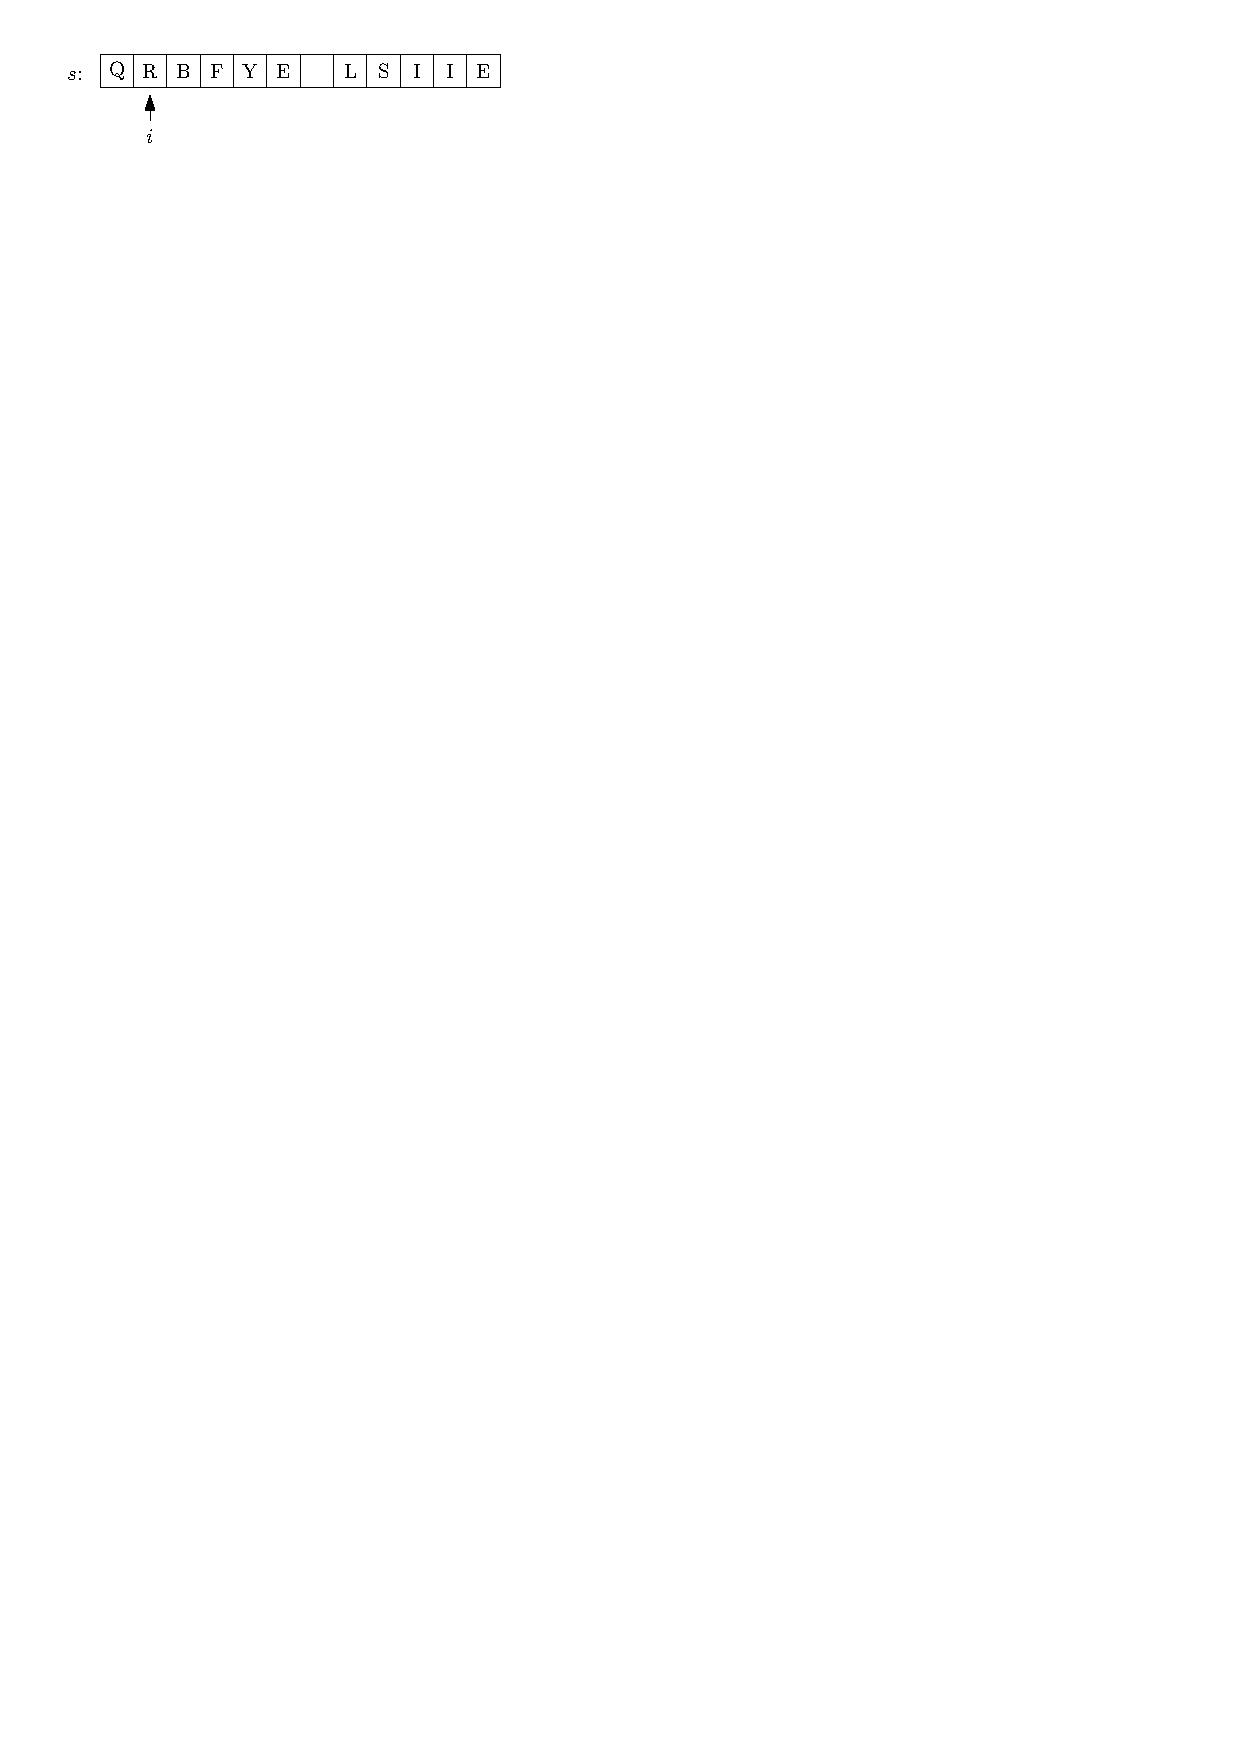
\includegraphics[scale=0.8]{01/figs/pdvcrypt.pdf}
  \end{center}

  {\small
  Jeden krok dešifrování:
  \vspace{-1em}
  \begin{itemize}
    \item $s_i \gets \Big[ s_i + p_1 \times secret(\overbrace{s_{[i-2 .. i+2]}}^{\text{EQRBF}}) \Big] \ \mathrm{mod}\ |\Sigma|$
    \item $i \gets \Big[ i + p_2 \times secret(s_{[i-2 .. i+2]}) \Big] \ \mathrm{mod} \ |s|$
  \end{itemize}
  ... opakován $N$-krát
  }

  \vspace{1em}


  \textbf{Úkol:} Doimplementujte dešifrovací pravidlo do metody \texttt{decrypt} v souboru \texttt{PDVCrypt.cpp}.
\end{frame}

\begin{frame}[fragile]
  \frametitle{Šifra \texttt{PDVCrypt}}
  \begin{block}{Je následující tvrzení pravdivé?}
    Proces dešifrování řetězce zašifrovaného pomocí \texttt{PDVCrypt} lze snadno paralelizovat.
  \end{block}
  \pause
  \textcolor{BrickRed}{\bf Tvrzení není pravdivé.}
  Proč paralelní verze dešifrovacího algoritmu vůbec nefunguje?

  \pause
  \vspace{3em}\hrule
  Uvažujte množinu zašifrovaných řetězců, které máte za úkol dešifrovat.
  Mohli bychom využít více jader v tomto případě?
\end{frame}
}

% \begin{frame}[standout]
%   \begin{minipage}{0.4\linewidth}
%     \begin{center}
%       \textbf{\LARGE Díky za pozornost!}
%     \end{center}

%     \vspace{3em}

%     \raggedleft\small Budeme rádi za Vaši\\zpětnou vazbu! $\rightarrow$
%   \end{minipage}
%   \hfill
%   \begin{minipage}{0.5\linewidth}
%     % \vspace{4em}
%     \centering
\includegraphics[width=\linewidth]{01/figs/qr_feedback.pdf}
%   \end{minipage}
% \end{frame}

\framefeedback{https://forms.gle/RAkkWY2knrdG9qpY7}

\end{document}
